% LID ensemble flow with romanization
\documentclass[tikz,border=5pt]{standalone}
\usetikzlibrary{arrows.meta,shapes.geometric}
\begin{document}
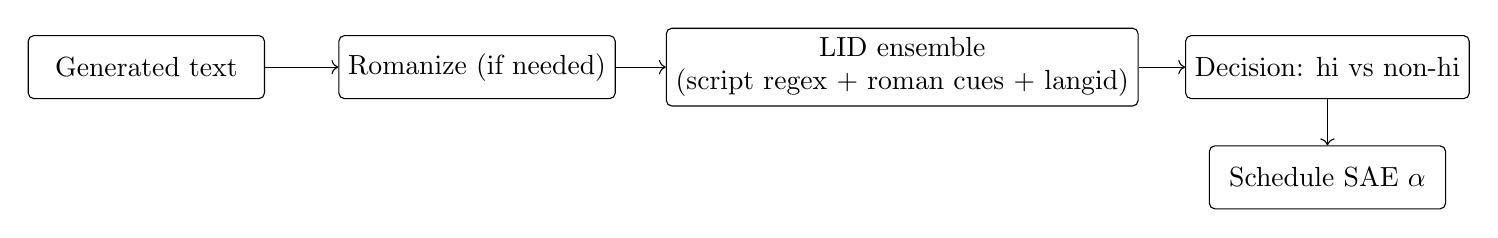
\begin{tikzpicture}[
  node distance=10mm and 14mm,
  box/.style={draw, rounded corners=2pt, minimum width=30mm, minimum height=8mm, align=center},
  line/.style={->}
]
\node[box] (gen) at (0,0) {Generated text};
\node[box] (rom) at (42mm,0) {Romanize (if needed)};
\node[box] (lid) at (96mm,0) {LID ensemble\\(script regex + roman cues + langid)};
\node[box] (dec) at (150mm,0) {Decision: hi vs non-hi};
\node[box] (sched) at (150mm,-14mm) {Schedule SAE $\alpha$};

\draw[line] (gen) -- (rom);
\draw[line] (rom) -- (lid);
\draw[line] (lid) -- (dec);
\draw[line] (dec) -- (sched);
\end{tikzpicture}
\end{document}

